\documentclass[a4paper, 12pt]{report}		% general format

%%%% Charset
\usepackage{cmap}							% make PDF files searchable and copyable
\usepackage[utf8]{inputenc}					% accept different input encodings
\usepackage[T2A]{fontenc}					% russian font
\usepackage[russian]{babel}					% multilingual support (T2A)

%%%% Graphics
\usepackage[dvipsnames]{xcolor}			% driver-independent color extensions
\usepackage{graphicx}						% enhanced support for graphics
\usepackage{wrapfig}						% pro­duces fig­ures which text can flow around

%%%% Math
\usepackage{amsmath}						% Amer­i­can Math­e­mat­i­cal So­ci­ety (AMS) math fa­cil­i­ties
\usepackage{amsfonts}						% fonts from the AMS
\usepackage{amssymb}						% additional math symbols

%%%% Ty­po­grapy (don't forget about cm-super)
\usepackage{microtype}						% sublim­i­nal re­fine­ments to­wards ty­po­graph­i­cal per­fec­tion
\linespread{1.3}							% line spacing
\usepackage[left=2.5cm, right=1.5cm, top=2.5cm, bottom=2.5cm]{geometry}
\setlength{\parindent}{0pt}					% we don't want any paragraph indentation
\renewcommand{\chaptername}{}

%%%% Other
\usepackage{url}							% ver­ba­tim with URL-sen­si­tive line breaks
%\DeclareUnicodeCharacter{00A0}{~}

%------------------------------------------------------------------------------
\usepackage{listings}						% type­set source code list­ings

% Цвета для кода
\definecolor{string}{HTML}{101AF9}			% цвет строк в коде
\definecolor{comment}{HTML}{3F7F5F}		% цвет комментариев в коде
\definecolor{keyword}{HTML}{5F1441}		% цвет ключевых слов в коде
\definecolor{morecomment}{HTML}{8000FF}	% цвет include и других элементов в коде
\definecolor{captiontext}{HTML}{FFFFFF}	% цвет текста заголовка в коде
\definecolor{captionbk}{HTML}{999999}		% цвет фона заголовка в коде
\definecolor{bk}{HTML}{FFFFFF}				% цвет фона в коде
\definecolor{frame}{HTML}{999999}			% цвет рамки в коде

% Настройки отображения кода
\lstset{
	language=C++,							% Язык кода по умолчанию
	morekeywords={*,...},					% если хотите добавить ключевые слова, то добавляйте
	% Цвета
	keywordstyle=\color{keyword}\ttfamily\bfseries,
	stringstyle=\color{string}\ttfamily,
	commentstyle=\color{comment}\ttfamily\itshape,
	morecomment=[l][\color{morecomment}]{\#},
	% Настройки отображения
	breaklines=true,						% Перенос длинных строк
	basicstyle=\ttfamily\footnotesize,		% Шрифт для отображения кода
	backgroundcolor=\color{bk},				% Цвет фона кода
	%frame=lrb,xleftmargin=\fboxsep,xrightmargin=-\fboxsep, % Рамка, подогнанная к заголовку
	frame=tblr								% draw a frame at all sides of the code block
	rulecolor=\color{frame},				% Цвет рамки
	tabsize=2,								% tab space width
	showstringspaces=false,					% don't mark spaces in strings
	% Настройка отображения номеров строк. Если не нужно, то удалите весь блок
	numbers=left,							% Слева отображаются номера строк
	stepnumber=1,							% Каждую строку нумеровать
	numbersep=5pt,							% Отступ от кода
	numberstyle=\small\color{black},		% Стиль написания номеров строк
	% Для отображения русского языка
	extendedchars=true,
	literate={Ö}{{\"O}}1
	 	{Ä}{{\"A}}1
	 	{Ü}{{\"U}}1
		{ß}{{\ss}}1
		{ü}{{\"u}}1
		{ä}{{\"a}}1
		{ö}{{\"o}}1
		{~}{{\textasciitilde}}1
		{а}{{\selectfont\char224}}1
		{б}{{\selectfont\char225}}1
		{в}{{\selectfont\char226}}1
		{г}{{\selectfont\char227}}1
		{д}{{\selectfont\char228}}1
		{е}{{\selectfont\char229}}1
		{ё}{{\"e}}1
		{ж}{{\selectfont\char230}}1
		{з}{{\selectfont\char231}}1
		{и}{{\selectfont\char232}}1
		{й}{{\selectfont\char233}}1
		{к}{{\selectfont\char234}}1
		{л}{{\selectfont\char235}}1
		{м}{{\selectfont\char236}}1
		{н}{{\selectfont\char237}}1
		{о}{{\selectfont\char238}}1
		{п}{{\selectfont\char239}}1
		{р}{{\selectfont\char240}}1
		{с}{{\selectfont\char241}}1
		{т}{{\selectfont\char242}}1
		{у}{{\selectfont\char243}}1
		{ф}{{\selectfont\char244}}1
		{х}{{\selectfont\char245}}1
		{ц}{{\selectfont\char246}}1
		{ч}{{\selectfont\char247}}1
		{ш}{{\selectfont\char248}}1
		{щ}{{\selectfont\char249}}1
		{ъ}{{\selectfont\char250}}1
		{ы}{{\selectfont\char251}}1
		{ь}{{\selectfont\char252}}1
		{э}{{\selectfont\char253}}1
		{ю}{{\selectfont\char254}}1
		{я}{{\selectfont\char255}}1
		{А}{{\selectfont\char192}}1
		{Б}{{\selectfont\char193}}1
		{В}{{\selectfont\char194}}1
		{Г}{{\selectfont\char195}}1
		{Д}{{\selectfont\char196}}1
		{Е}{{\selectfont\char197}}1
		{Ё}{{\"E}}1
		{Ж}{{\selectfont\char198}}1
		{З}{{\selectfont\char199}}1
		{И}{{\selectfont\char200}}1
		{Й}{{\selectfont\char201}}1
		{К}{{\selectfont\char202}}1
		{Л}{{\selectfont\char203}}1
		{М}{{\selectfont\char204}}1
		{Н}{{\selectfont\char205}}1
		{О}{{\selectfont\char206}}1
		{П}{{\selectfont\char207}}1
		{Р}{{\selectfont\char208}}1
		{С}{{\selectfont\char209}}1
		{Т}{{\selectfont\char210}}1
		{У}{{\selectfont\char211}}1
		{Ф}{{\selectfont\char212}}1
		{Х}{{\selectfont\char213}}1
		{Ц}{{\selectfont\char214}}1
		{Ч}{{\selectfont\char215}}1
		{Ш}{{\selectfont\char216}}1
		{Щ}{{\selectfont\char217}}1
		{Ъ}{{\selectfont\char218}}1
		{Ы}{{\selectfont\char219}}1
		{Ь}{{\selectfont\char220}}1
		{Э}{{\selectfont\char221}}1
		{Ю}{{\selectfont\char222}}1
		{Я}{{\selectfont\char223}}1
		{і}{{\selectfont\char105}}1
		{ї}{{\selectfont\char168}}1
		{є}{{\selectfont\char185}}1
		{ґ}{{\selectfont\char160}}1
		{І}{{\selectfont\char73}}1
		{Ї}{{\selectfont\char136}}1
		{Є}{{\selectfont\char153}}1
		{Ґ}{{\selectfont\char128}}1
}

% Для настройки заголовка кода
\usepackage{caption}
\DeclareCaptionFont{white}{\color{сaptiontext}}
\DeclareCaptionFormat{listing}{\parbox{\linewidth}{\colorbox{сaptionbk}{\parbox{\linewidth}{#1#2#3}}\vskip-4pt}}
%\captionsetup[lstlisting]{format=listing,labelfont=white,textfont=white}
\renewcommand{\lstlistingname}{Листинг} % Переименование Listings в нужное именование структуры

%------------------------------------------------------------------------------
\begin{document}

\begin{titlepage}
\thispagestyle{empty}

\begin{center}
Санкт-Петербургский государственный политехнический университет \\
Институт Информационных Технологий и Управления \\*
Кафедра компьютерных систем и программных технологий \\*
\hrulefill
\end{center}

\vspace{18em}

\begin{center}
\Large Отчет по расчетной работе № 1 \\ по предмету «Системное программное обеспечение» \\
\end{center}

\vspace{1em}

% \linebreak
\begin{center}
\textsc{\textbf{Обработка исключений в ОС Windows}}
\end{center}

\vspace{16em}

\begin{flushleft}
Работу выполнил студент гр. 53501/3\hrulefill Мартынов С. А. \\
\vspace{1.5em}
Работу принял преподаватель \hrulefill Душутина Е. В. \\
\end{flushleft}

\vspace{\fill}

\begin{center}
Санкт-Петербург \\
2014
\end{center}

\end{titlepage}
%------------------------------------------------
\setcounter{page}{2}
\tableofcontents
%------------------------------------------------

\chapter*{Постановка задачи}
\addcontentsline{toc}{chapter}{Постановка задачи}

\begin{enumerate}
	\item Сгенерировать и обработать исключения с помощью функций WinAPI;
	\item Получить код исключения с помощью функции GetExceptionCode.
		\begin{itemize}
		\item Использовать эту функции в выражении фильтре;
		\item Использовать эту функцию в обработчике.
		\end{itemize}
	\item Создать собственную функцию-фильтр;
	\item Получить информацию об исключении с помощью функции GetExceptionInformation; сгенерировать исключение с помощью функции RaiseException;
	\item Использовать функции UnhandledExceptionFilter и SetUnhandledExceptionFilter для необработанных исключений;
	\item Обработать вложенные исключения;
	\item Выйти из блока \_\_try с помощью оператора goto;
	\item Выйти из блока \_\_try с помощью оператора \_\_leave;
	\item Преобразовать структурное исключение в исключение языка С, используя функцию translator;
	\item Использовать финальный обработчик finally;
	\item Проверить корректность выхода из блока \_\_try с помощью функции AbnormalTermination в финальном обработчике \_\_finally.
\end{enumerate}

На каждый пункт представить отдельную программу, специфический код, связанный с особенностями генерации заданного исключения структурировать в отдельный элемент (функцию, макрос или иное).

\vspace{1em}
В данной работе рассматриваются следующие исключения:
\begin{itemize}
\item \textbf{EXCEPTION\_FLT\_DIVIDE\_BY\_ZERO} - поток попытался сделать деление на ноль с плавающей точкой;
\item \textbf{EXCEPTION\_FLT\_OVERFLOW} - переполнение при операции над числами с плавающей точкой.
\end{itemize}

\vspace{1em}
Все результаты, представленные в данном отчёте получены с использованием Microsoft Windows 7 Ultimate Service Pack 1 64-bit (build 7601). Для разработки использовалась Microsoft Visual Studio Express 2013 for Windows Desktops (Version 12.0.30723.00 Update 3). В качестве отладчика использовался Microsoft WinDbg (release 6.3.9600.16384).

\vspace{1em}
Исходный код всех представленных листингов доступен по адресу \\ \url{https://github.com/SemenMartynov/SPbPU_SystemProgramming}.
%------------------------------------------------

\chapter*{Исключения с помощью WinAPI}
\addcontentsline{toc}{chapter}{Исключения с помощью WinAPI}

Задачей этого раздела является генерирование и обработка исключений с помощью функций WinAPI.

В листинге 1 показана работа с исключениями. В зависимости от параметра, передаваемого при запуске, вызывается либо исключение деления на ноль, либо переполнение разрядной сетки при работе с типом float. Особо стоит обратить внимание на две вещи: изначально, все ошибки типа float маскируются, и для получения исключений нужно от этого маскирования избавиться (см. стр. 64-65); кроме того, операции с плавающими точками выполняются асинхронно, и нужно на этапе компиляции отключить расширения векторизации.

В 69-й строке используется квалификатор volatile, это помогает обмануть статический анализатор среды разработки (visual studio), который честно сигнализирует о явной ошибке (делении на ноль) и не позволяет собрать программу.

\lstinputlisting[language=C++, caption={Генерация и обработка исключения с помощью функций WinAPI}]
{../../src/ExceptionsProcessing/WinAPI/main.cpp}


Если запустить этот код в отладчике (рисунок 2), и пройти его по шагам, то можно увидеть, как управление с 73-й строки (где происходит исключительная ситуация),  передаётся на 88-ю (в которой ожидается исключение), а потом на 93-ю (т.е. обратной передачи управления не происходит).

Произведём три запуска, первый раз без аргументом (для демонстрации зависимости исключения от передаваемого аргумента), второй раз с аргументом "\-d" (DIVIDE\_BY\_ZERO) и третий раз с аргументом "\-o" (FLT\_OVERFLOW). Как видно на рисунке 1, первый запуск не дал результатов, второй и третий привёл к исключительной ситуации.

\begin{figure}[h!]
\centering
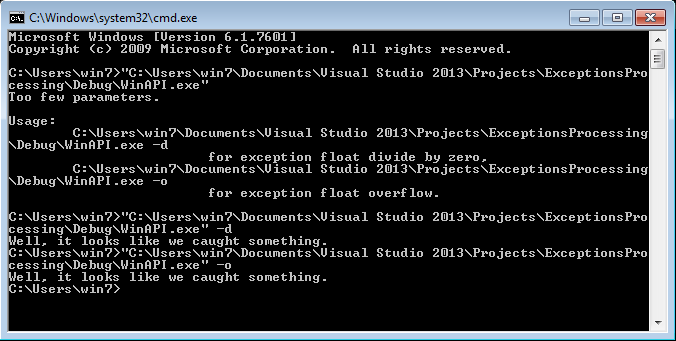
\includegraphics[scale=0.95]{res/001}
\caption{Запуск программы, генерирующей исключения средствами WinAPI.}
\end{figure}

Во время второго и третьего запуска, управление сразу после исключения передавалось на 88-ю строку, это можно видеть по листингу 2, содержащему лог работы программы. Запись из 74-й и 82-й строки в нём отсутствует, т.к. управление до этих строк не дошло.

\lstinputlisting[language={},caption={Генерация и обработка исключения с помощью функций WinAPI}]{res/WinAPI.log}

Передачу управления можно видеть и по средствам отладчика. В правом нижнем углу показан стек. В данном случе глубина стека не достаточно большая для наглядного изучения поиска обработчика, но вызов обработчика на нём виден.

\begin{figure}[h!]
\centering
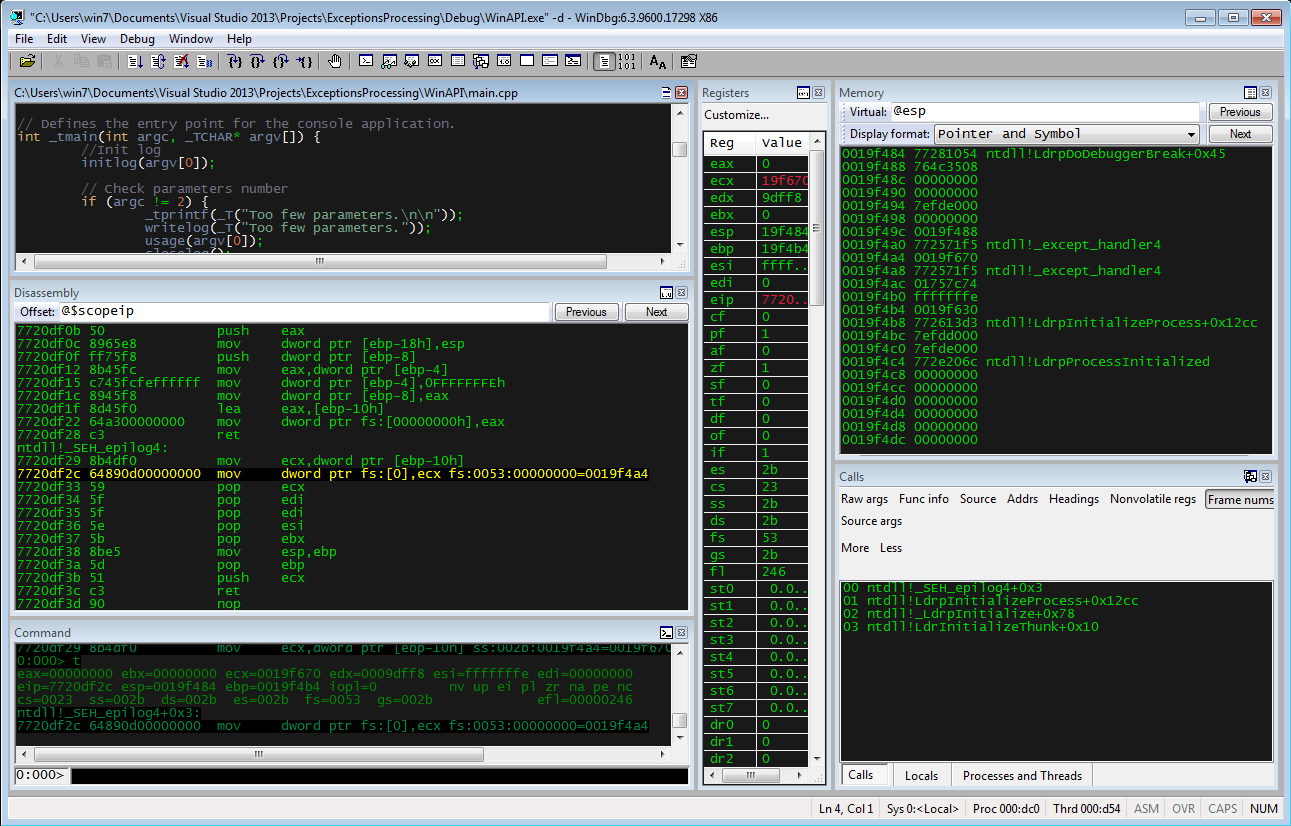
\includegraphics[scale=0.5]{res/002}
\caption{Запуск WinAPI.exe под отладчиком WinDbg.}
\end{figure}

Благородя тому, что исключение было обработано, оно не дошло до уровня операционной системы, и не было отражено в системном журнале.

%------------------------------------------------

\chapter*{Использование GetExceptionCode}
\addcontentsline{toc}{chapter}{Использование GetExceptionCode}

Функция GetExceptionCode позволяет получить код исключения, которое было сгенерировано в процессе работы программы (смотри листинг 3). В первом случае (строка 79) она участвует в сравнении с макро-константной EXCEPTION\_FLT\_DIVIDE\_BY\_ZERO для определения подходящего обработчика для исключительного события. Во-втором случае (строка 98) она используется уже внутри обработчика, позволяя определить, что исключение вызвано переполнением при операции с типом float.

\lstinputlisting[language=C++, caption={Получение кода исключения с помощью функции GetExceptionCode}]
{../../src/ExceptionsProcessing/GetExceptionCode/main.cpp}

Таким образом, рассмотрены два способа фильтрации исключений - на уровне входа в блок \_\_except, либо уже непосредственно в обработчике (тогда в \_\_except ставится макро-константа EXCEPTION\_EXECUTE\_HANDLER, позволяющая принимать любые исключения). Далее будет рассмотрен более логичный способ фильтрации исключений специальной функцией.

Запуск под отладчиком показывает картину практически аналогичную предыдущему случаю, но есть разница в логе работы программы (листинг 4). На этот раз мы знаем какое исключение произошло и это фиксируем в логе.

\lstinputlisting[language={},caption={Генерация и обработка исключения с помощью функций WinAPI}]{res/GetExceptionCode.log}

%------------------------------------------------

\chapter*{Пользовательская функция-фильтр}
\addcontentsline{toc}{chapter}{Пользовательская функция-фильтр}

В листинге 5 представлена функция-фильтр, которая возвращает \\ EXCEPTION\_CONTINUE\_SEARCH только если исключение вызвано \\ EXCEPTION\_FLT\_DIVIDE\_BY\_ZERO или EXCEPTION\_FLT\_OVERFLOW.

\lstinputlisting[language=C++, caption={Использование собственной функции фильтра}]
{../../src/ExceptionsProcessing/FilterFunction/main.cpp}

При изучении работы программы под отладчиком, выяснилось что при возникновении исключения, управление не передаётся в то место, где определена функция-фильтр. Вероятно компилятор оптимизирует код и подставляет её целиком на место вызова. На рисунке 3 видна передача управления на обработку исключения после работы функции-фильтра.

\begin{figure}[h!]
\centering
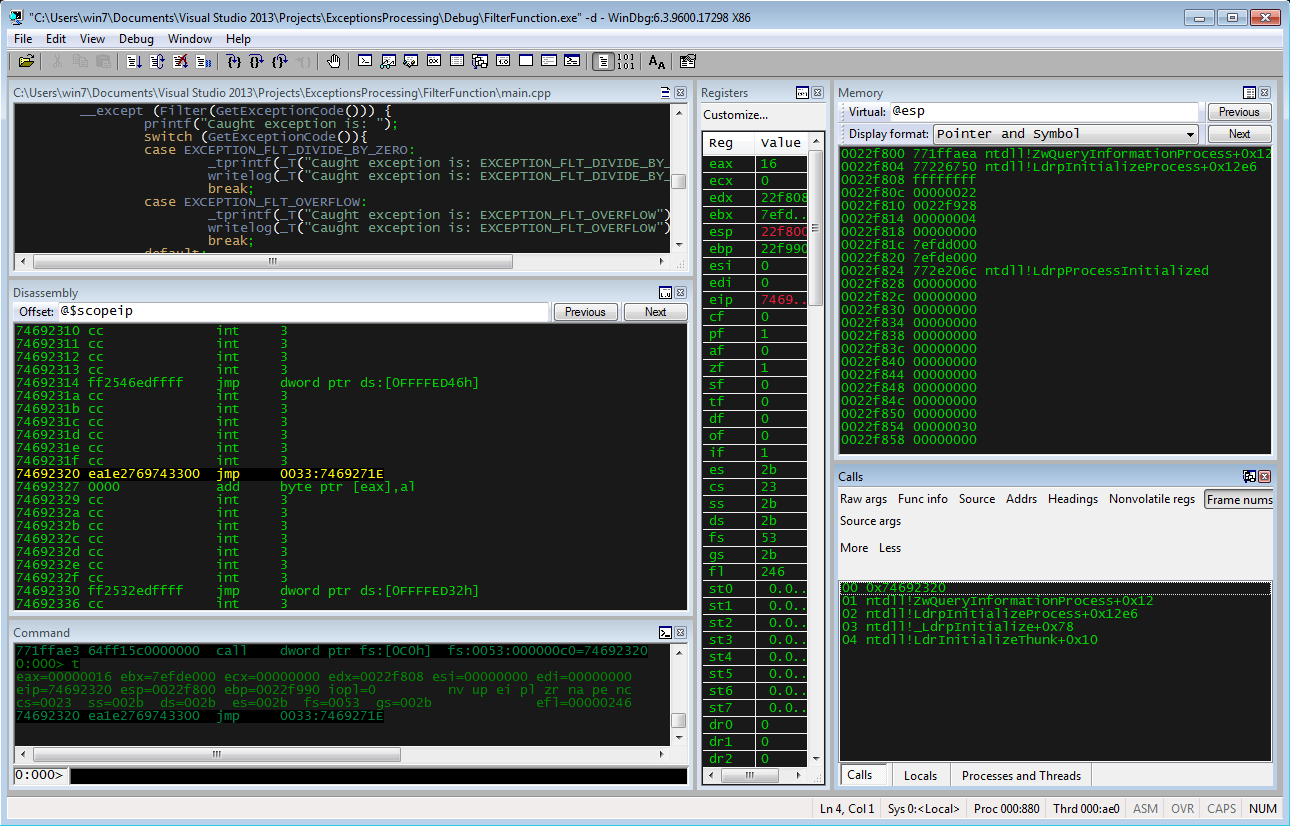
\includegraphics[scale=0.5]{res/003}
\caption{Передача управления обработчику, после отработки функции-фильтра}
\end{figure}

В обработчике фактически происходит только вызов функций логирования (листинг 6). Как и раньше, строки 75 и 83 оказываются пропущенными, т.к. после возбуждения исключения управление переходит обработчику, нарушая линейный порядок.

\lstinputlisting[language={},caption={Генерация и обработка исключения с помощью функций WinAPI}]{res/FilterFunction.log}

%------------------------------------------------

\chapter*{Использование RaiseException}
\addcontentsline{toc}{chapter}{Использование RaiseException}

Исключение можно возбудить не только в результате каких-то арифметических или логических операций, но и искучтвенным образом, вызвав функцию RaiseException. Она обладает 4-я параметрами, но наиболее важным является первый, который определяет тип возбуждаемого исключения. Работа этой функции показана в листинге 7.

\lstinputlisting[language=C++, caption={Программная генерация исключения при помощи функции RaiseException}]
{../../src/ExceptionsProcessing/RaiseException/main.cpp}

Информацию об исключении можно получить из функции GetExceptionInformation, которая, в действительности, никакой информацией не владеет но возвращает указатель на структуру EXCEPTION\_POINTERS. В свою очередь, эта структура содержит два указателя на ExceptionRecord и на ContextRecord, в которых уже находится информация об исключении.

\begin{figure}[h!]
\centering
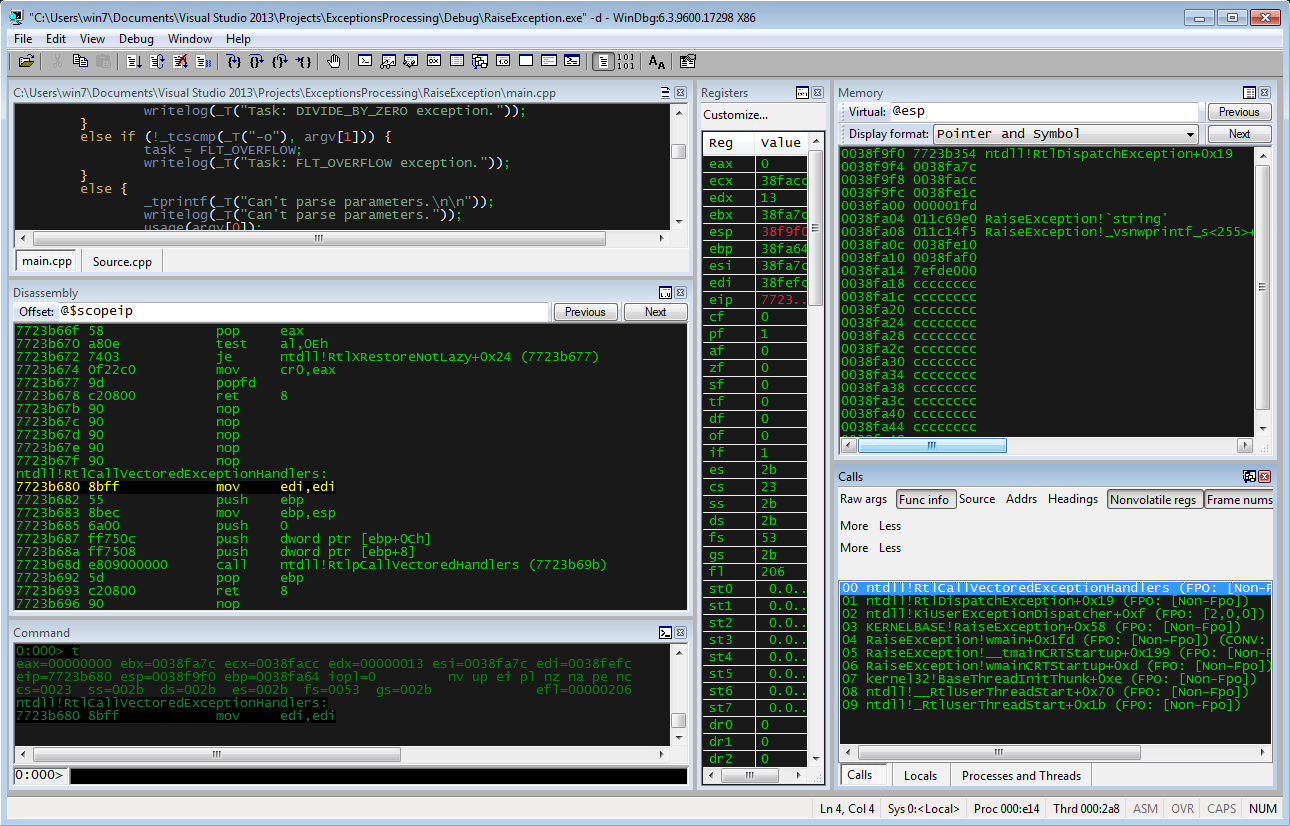
\includegraphics[scale=0.5]{res/005}
\caption{Информация об исключении доступна в процессе работы функции-фильтра}
\end{figure}

Важной особенностью функции GetExceptionlnformation является то, что ее можно вызывать только в функции-фильтре исключений, т.к. структуры CONTEXT, EXCEPTION\_RECORD и EXCEPTION\_POINTERS существуют лишь во время обработки фильтра исключения. В момент, когда управление переходит к обработчику исключений, эти данные в стеке разрушаются. На рисунке 4 показан момент получения информации о возникшем исключении. Обработчик исключения находится выше по стеку, и когда ему будет возвращено управление от функции фильтра стек уже будет зачищен.

\begin{figure}[h!]
\centering
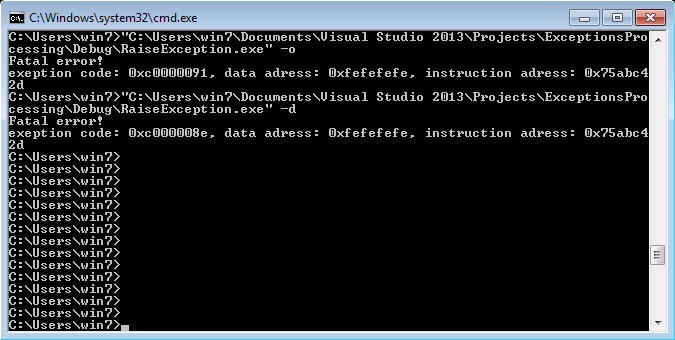
\includegraphics[scale=0.95]{res/004}
\caption{Передача управления обработчику, после отработки функции-фильтра}
\end{figure}

На рисунке 5 показан вызов программы, генерирующей исключения программным образом, а в листинге 8 представлен лог её работы.

\lstinputlisting[language={},caption={Программная генерация исключения и получение информации о нём}]{res/RaiseException.log}

%------------------------------------------------

\chapter*{Не обрабатываемые исключения}
\addcontentsline{toc}{chapter}{Не обрабатываемые исключения}

Если ни один из установленных программистом обработчиков не подошла для обработки исключения (либо программист вообще не установил ни один обработчик), то вызывается функция UnhandledExceptionFilter, которая выполняет проверку, запущен ли процесс под отладчиком, и информирует процесс, если отладчик доступен. Далее, функция вызывает фильтр умалчиваемого обработчика (который устанавливается функцией SetUnhandledExceptionFilter и который возвращает EXCEPTION\_EXECUTE\_HANDLER). Затем, в зависимости от настроек операционной системы, вызывается либо отладчик, либо функция NtRaiseHardError, которая отображает сообщение об ошибке. 

Листинг 9 показывает работу с UnhandledExceptionFilter. Возвращаемое значение определяется в строках 108 и 109.

\lstinputlisting[language=C++, caption={Необработанные исключения}]
{../../src/ExceptionsProcessing/UnhandleExceptionFilter/main.cpp}

Для начала запустим программу так, чтобы фильтр возвращал EXCEPTION\_EXECUTE\_HANDLER. Это считается нормальной ситуацией, и на рисунке 6 видно как происходит передача управления.

\begin{figure}[h!]
\centering
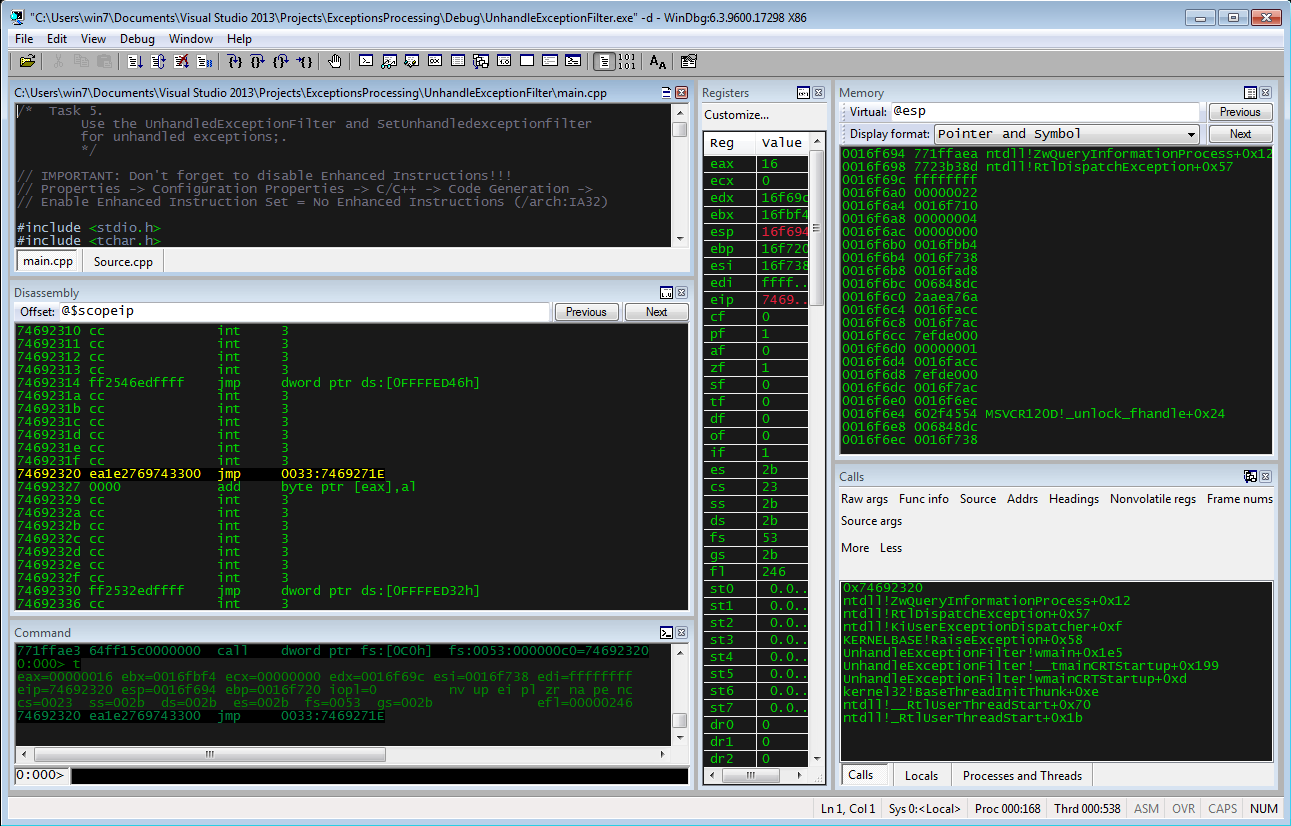
\includegraphics[scale=0.5]{res/006}
\caption{Нормальная обработка исключения через фильтр}
\end{figure}

Запустим программу ещё раз,  фильтр вернёт EXCEPTION\_CONTINUE\_SEARCH. Это событие будет передано операционной системе, и будет зафиксировано в системном журнале (рисунок 7). Что примечательно, обработчик успел выполнить свою задачу, информация об ошибке выведена на экран (рисунок 8) и сохранена в лог (листинг 10), системная ошибка возникла уже после.

\begin{figure}[h!]
\centering
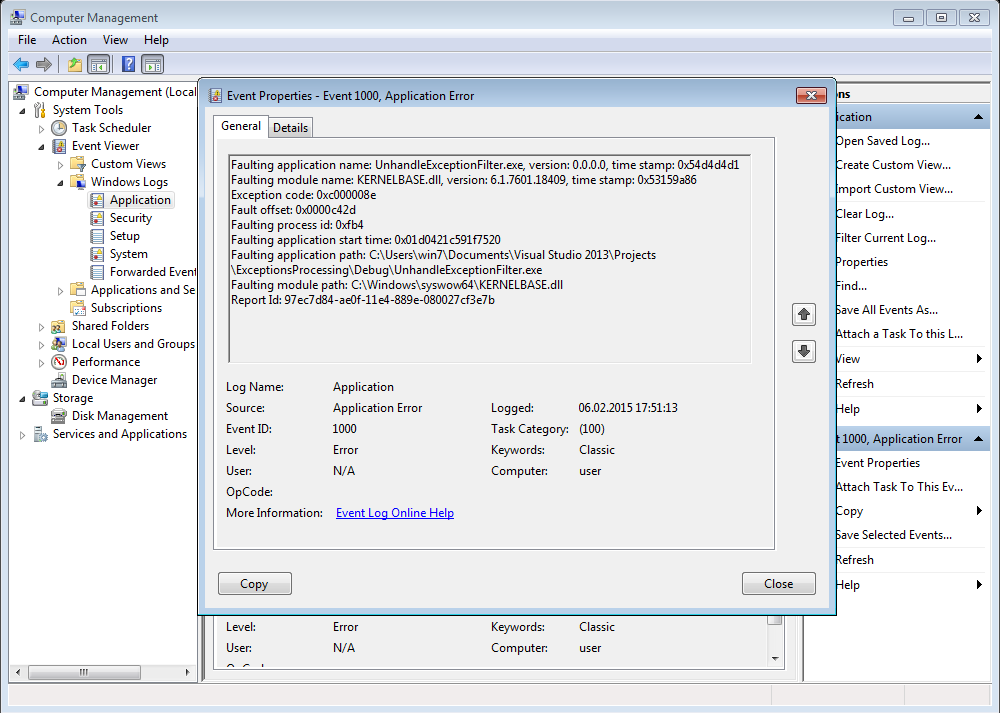
\includegraphics[scale=0.63]{res/007}
\caption{Исключение зафиксировано в системном журнале}
\end{figure}

\begin{figure}[h!]
\centering
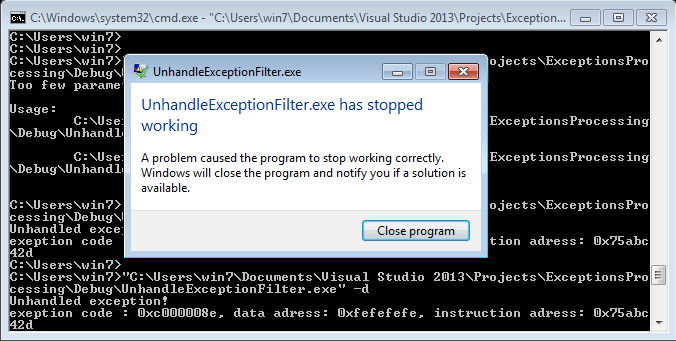
\includegraphics[scale=0.8]{res/008}
\caption{Обработчик успел выполниться до системной ошибки}
\end{figure}

В логе программы можно прочитать информацию о произошедшей исключительной ситуации. Вместе с тем, можно видеть, что программа не была завершена корректно, а дескриптер файла-лога не был закрыт.

\lstinputlisting[language={},caption={Обработчик успел сохранить данные об исключении}]{res/UnhandleExceptionFilter.log}

Из рассмотренного примера становится видно, что возврат EXCEPTION\_EXECUTE\_HANDLER является более предпочитаемым результатом, т.к. исключение нужно обрабатывать там, где оно возникло.

%------------------------------------------------

\chapter*{Вложенные исключения}
\addcontentsline{toc}{chapter}{Вложенные исключения}

Листинг 11 показывает, как происходит передача исключения, в поисках подходящего обработчика. Самым ближайшим (по стеку) обработчиком для исключения, вызванного делением на 0, является обработчик из 40-й строки. Но там стоит ограничение, позволяющее обрабатывать только исключения, вызванные переполнением. В результате обработка этого исключения передаётся в 48-ю строку, хотя этот обработчик дальше по стеку.

\lstinputlisting[language=C++, caption={Вложенные исключения}]
{../../src/ExceptionsProcessing/NestedException/main.cpp}

Запуск отладчика подтвердил ожидаемый результат - поиск подходящего обработчика для исключения происходит снизу вверх. В начале проверяется ближайший обработчик (на рисунке 9 отрабатывает фильтр ближайшего обработчика исключения). Эта проверка вернёт EXCEPTION\_CONTINUE\_SEARCH для продолжения поиска более подходящего обработчика и передачи управления дальше по стеку.

\begin{figure}[h!]
\centering
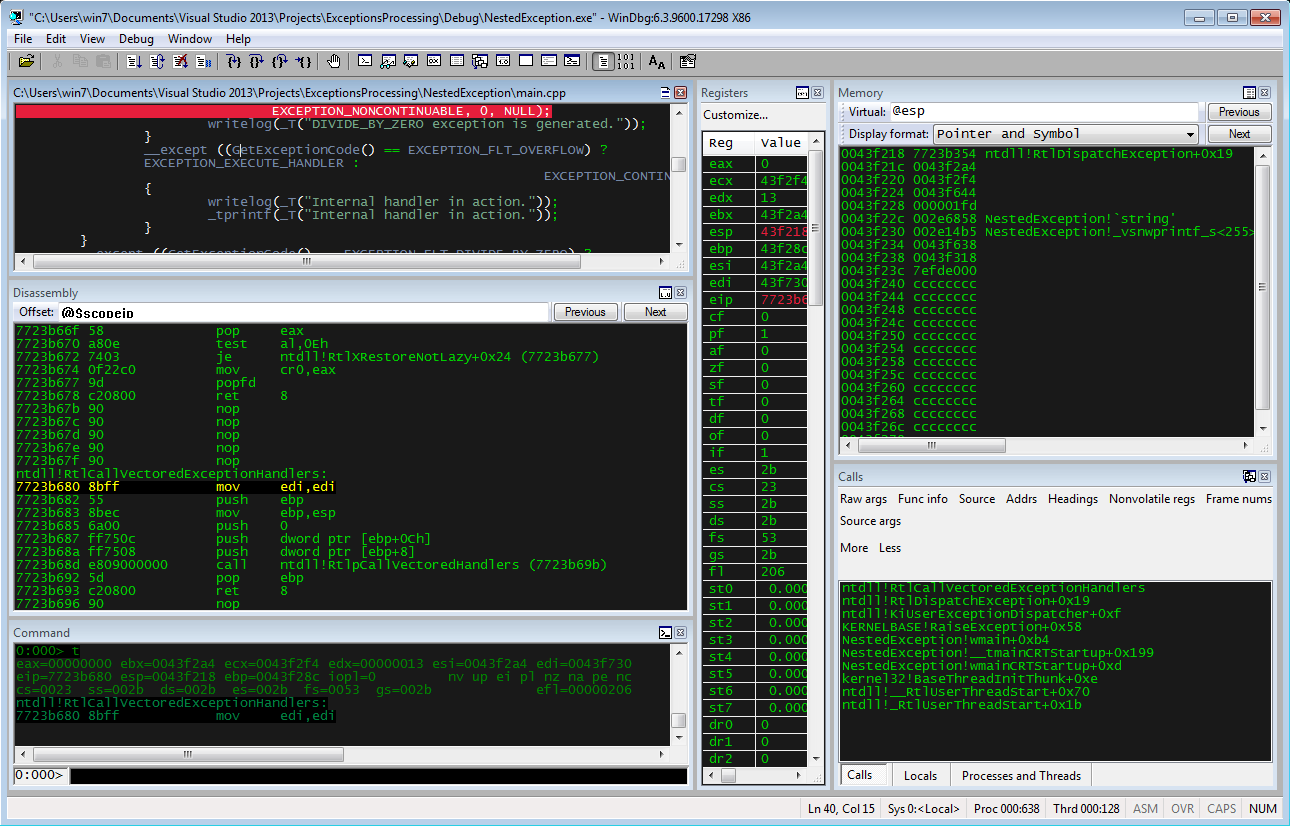
\includegraphics[scale=0.50]{res/009}
\caption{Проверка условий обработчика исключения}
\end{figure}

При этом создаётся опасность утечки ресурсов, поэтому желательно обрабатывать исключительные ситуации в месте их возникновения. Протокол работы программы показан в листинге 12.

\lstinputlisting[language={},caption={Обработчик успел сохранить данные об исключении}]{res/NestedException.log}
%------------------------------------------------

\chapter*{Выход при помощи goto}
\addcontentsline{toc}{chapter}{Выход при помощи goto}

Использование goto считается дурной практикой по целому ряду причин. В листинге 13, благодаря goto управление со строки 35 передаётся сразу на строку 46. Таким образом осуществляется выход из блока \_\_try без возбуждения и обработки исключения.

\lstinputlisting[language=C++, caption={Выход из блока охраняемого кода при помощи goto}]
{../../src/ExceptionsProcessing/Goto/main.cpp}

\begin{figure}[h!]
\centering
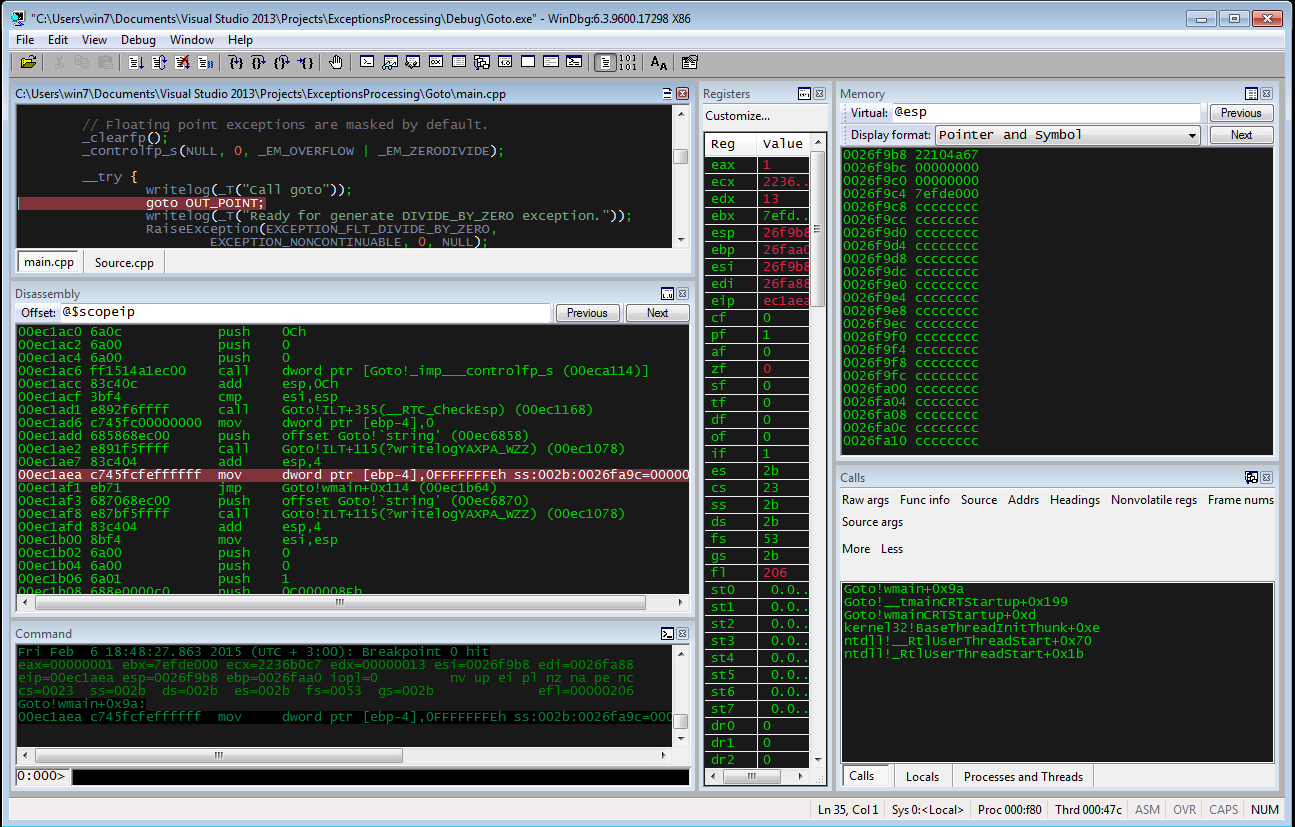
\includegraphics[scale=0.50]{res/010}
\caption{Переход по goto}
\end{figure}

На рисунке 10 видно, что как только достигнута строка с оператором goto, осуществляется безусловный переход к метке. Протокол работы программы (листинг 14) подтверждает, что до возбуждения исключения управление не дошло: после записи  логе из 34-й строки идёт запись из 47-й, таким образом строки 36-39 пропущены.

\lstinputlisting[language={},caption={Переход по оператору goto}]{res/Goto.log}

Использование goto может привести к утечкам памяти в процессе раскрутки стека, в то же время он позволяет сделать переход сразу через несколько участков кода. Таким образом, сфера применения goto достаточно узкая, и требует достаточно чёткого понимания.
%------------------------------------------------

\chapter*{Выход при помощи \_\_leave}
\addcontentsline{toc}{chapter}{Выход при помощи \_\_leave}

Листинг 15 похож на листинг 13, но за пределы охраняемого фрейма кода помогает выйти на этот раз \_\_leave. Оператор \_\_leave более эффективен, поскольку не вызывает разрушение стека.

\lstinputlisting[language=C++, caption={Выход из блока охраняемого кода при помощи \_\_leave}]
{../../src/ExceptionsProcessing/Leave/main.cpp}

\begin{figure}[h!]
\centering
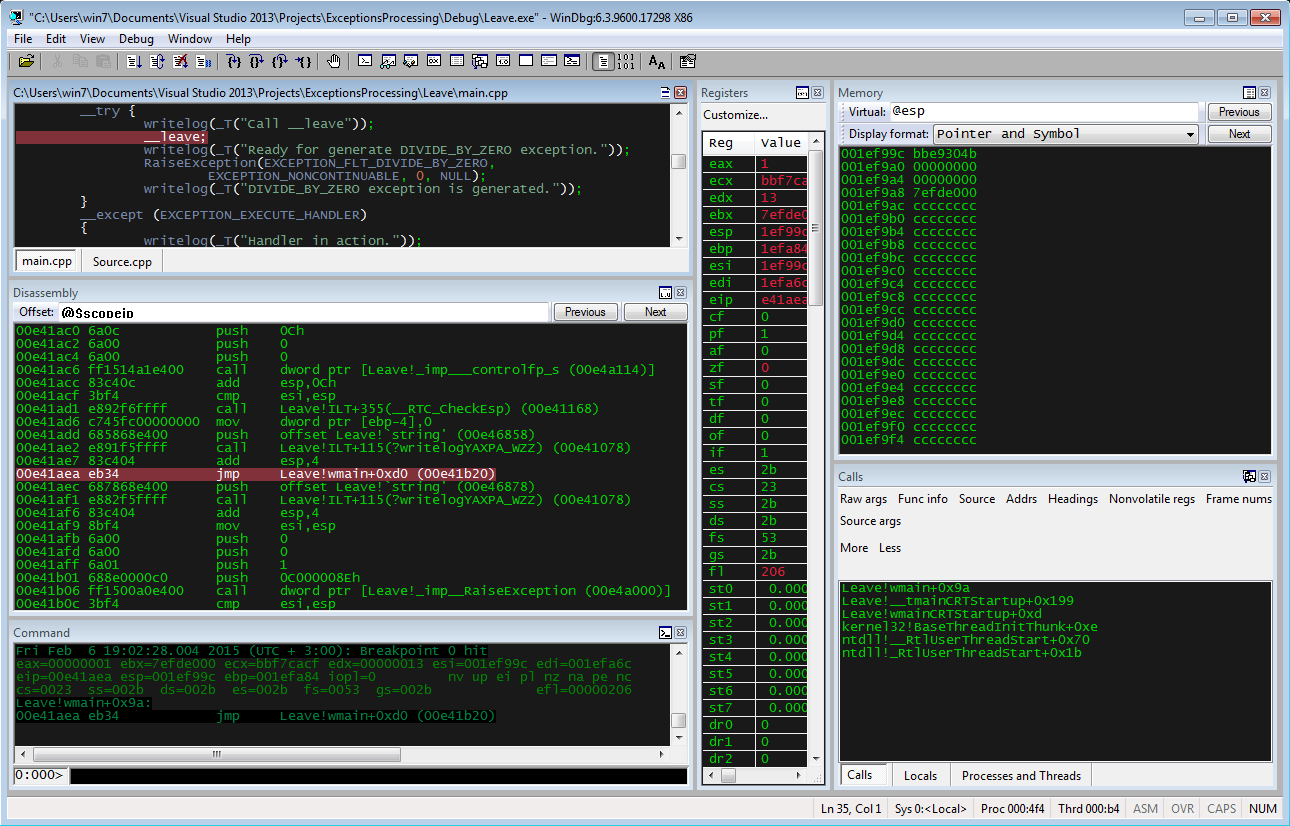
\includegraphics[scale=0.50]{res/011}
\caption{Переход по \_\_leave}
\end{figure}

\lstinputlisting[language={},caption={Переход по оператору \_\_leave}]{res/Leave.log}

Результат использования \_\_leave — переход в конец блока try (грубо говоря, это можно рассматривать это как goto переход на закрывающую фигурную скобку блока try и вход в блок finally естественным образом). По сути, результат прежний (если смотреть на листинг 16), но метод его достижения отличается -- этот способ считается более правильным, т.к. не приводит к раскрутке стека.

После перехода выполняется обработчик завершения. Хотя для получения того же результата можно использовать оператор goto, он (оператор goto) приводит к освобождению стека. Одним из применений этого оператора является трассировка программ.

%------------------------------------------------

\chapter*{Преобразование SEH в C++ исключение}
\addcontentsline{toc}{chapter}{Преобразование SEH в C++ исключение}

Листинг 17 показывает встраивание SEH в механизм исключений C/С++. Для этого необходимо включить соответствующие опции в компиляторе (/EHa).

\lstinputlisting[language=C++, caption={Трансформация исключений}]
{../../src/ExceptionsProcessing/Translator/main.cpp}

На рисунке 12 видна передача управления от генерации исключения в ядре к созданию пользовательского исключения. Листинг 18 показывает, какие участи кода были задействованы и в каком порядке.

\begin{figure}[h!]
\centering
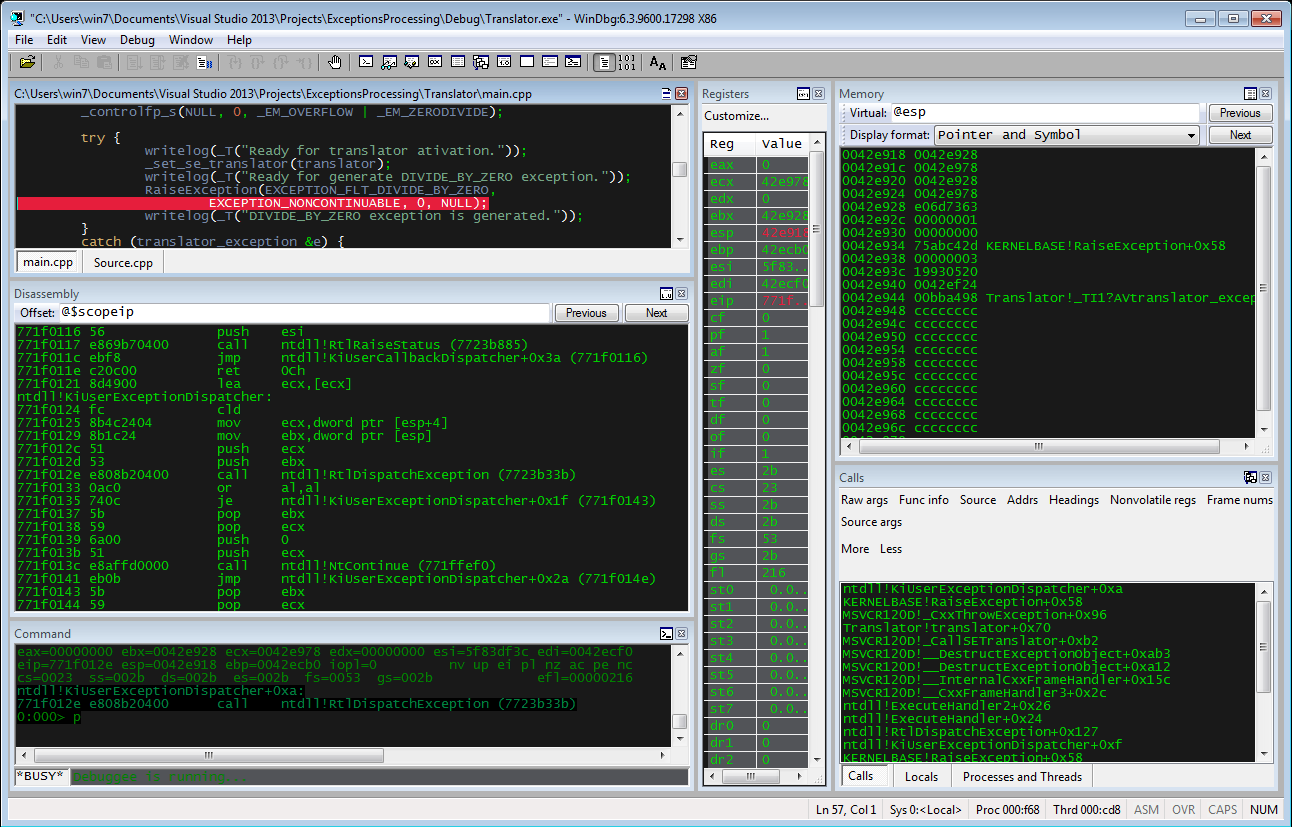
\includegraphics[scale=0.50]{res/012}
\caption{Передача управления коду создания пользовательского исключения}
\end{figure}

\lstinputlisting[language={},caption={Результат работы Translator.exe}]{res/Translator.log}

Если проследить за передачей управления по стеку вызовов, то сразу после возбуждения исключения в 56-й строке, управление передаётся транслятору, где генерируется привычное С++-исключения (в данном случае используется собственный класс исключения, определённый в 33-й строке), и только после этого в блок catch, где происходит обработка исключения.

Этот механизм способен обеспечить взаимодействие SEH с другими языками и системами.
%------------------------------------------------

\chapter*{Финальный обработчик finally}
\addcontentsline{toc}{chapter}{Финальный обработчик finally}

В листинге 19 исключение как таковое отсутствует, но есть охраняемый блок кода, и блок \_\_finally, управление в который будет передано в любой ситуации.

\lstinputlisting[language=C++, caption={Исполнение кода в блоке \_\_finally}]
{../../src/ExceptionsProcessing/Finally/main.cpp}

\begin{figure}[h!]
\centering
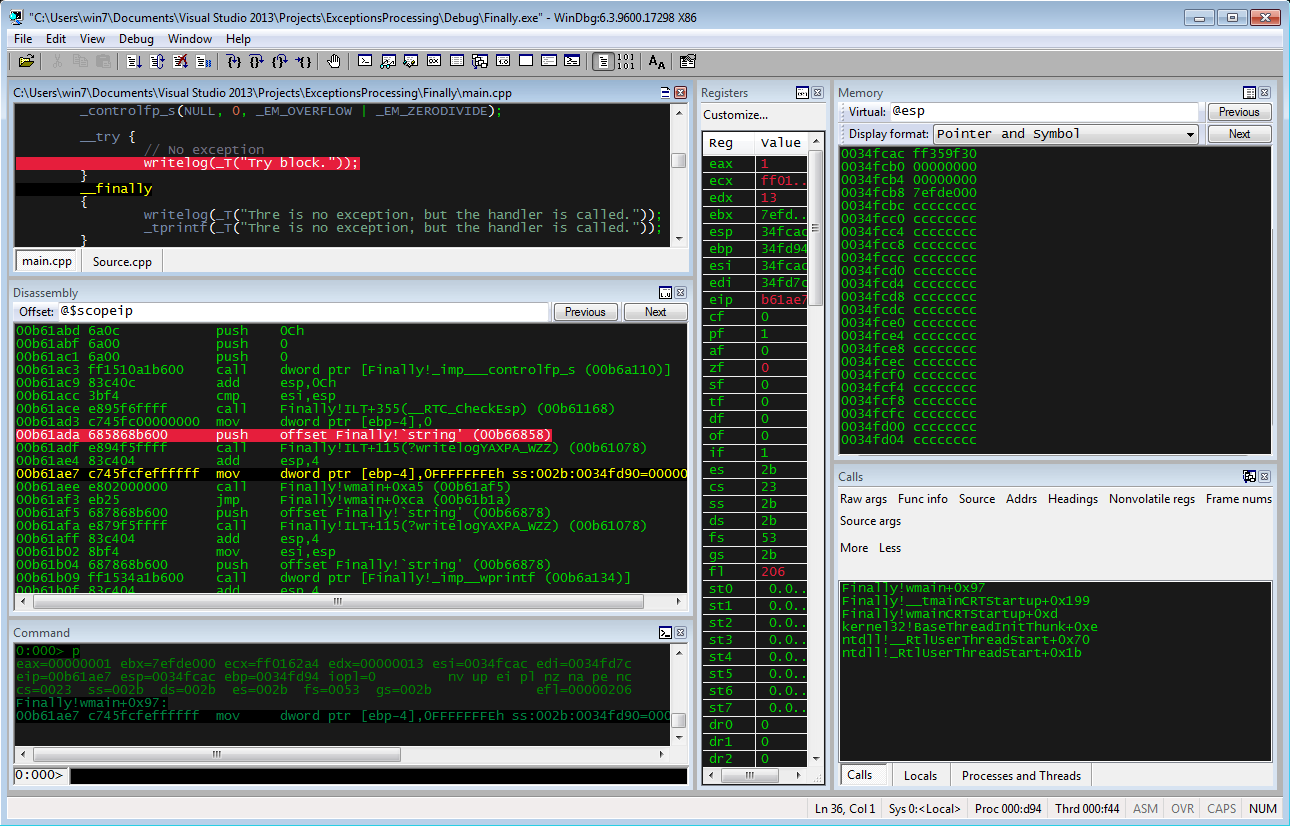
\includegraphics[scale=0.50]{res/013}
\caption{Переход в блок finally}
\end{figure}

\lstinputlisting[language={},caption={Результат работы Finally.exe}]{res/Finally.log}

Вместо передачи управления обратно в программу, управление передаётся в блок \_\_finally (рисунок 13). Более того, управление туда будет передано даже если блок защищаемого кода будет пуст. Листинг 20 показывает порядок исполнения кода.

Похожие механизмы есть в других распространённых языках программирования, они позволяют обеспечить строгие гарантии исключений, и не допустить нахождение объекта в не консистентном состоянии.
\newpage
%------------------------------------------------

\chapter*{Использование функции AbnormalTermination}
\addcontentsline{toc}{chapter}{Использование функции AbnormalTermination}

В листинге 21 сравниваются два механизма из блока \_\_try. Благодаря тому, что управление будет передано блоку \_\_finally в любом случае, оказывается удобно в этом блоке проверять корректность выхода из блока \_\_try (при помощи функции AbnormalTermination), и, в случае необходимости, корректно освобождать захваченные ресурсы.

\lstinputlisting[language=C++, caption={Проверка корректности выхода из блока \_\_try}]
{../../src/ExceptionsProcessing/AbnormalTermination/main.cpp}

\begin{figure}[h!]
\centering
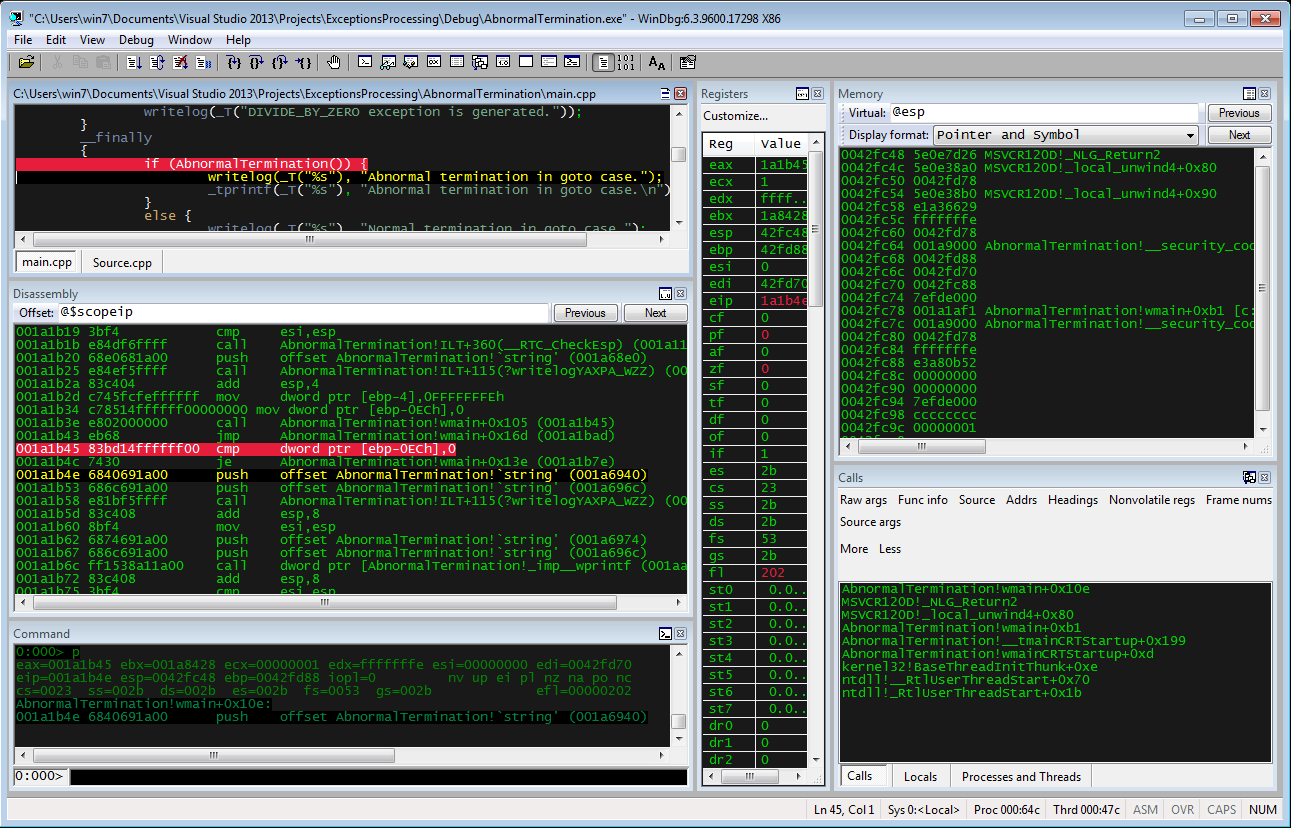
\includegraphics[scale=0.50]{res/014}
\caption{Выход из защищаемого блока по goto}
\end{figure}

\begin{figure}[h!]
\centering
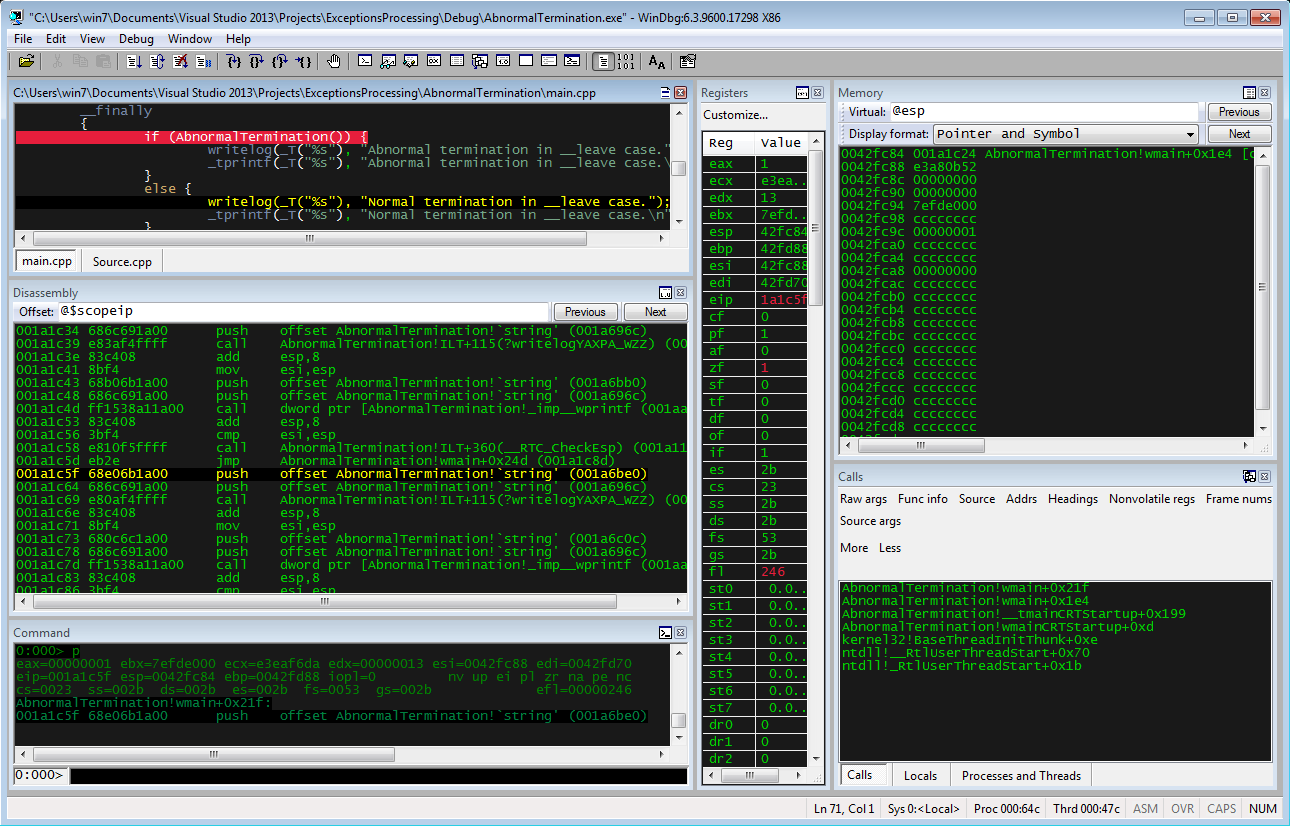
\includegraphics[scale=0.50]{res/015}
\caption{Выход из защищаемого блока по \_\_leave}
\end{figure}


Функция AbnormalTermination() позволяет определить на сколько правильным был выход из защищаемого кода в случае с goto (рисунок 14) и \_\_leave (рисунок 15). Протокол работы программы представлен в листинге 22.

В зависимости от этого принимается решение об освобождении захваченных ресурсов, но если по какой-то причине нужно выйти из защищаемого блока (хотя причина такой необходимости не очевидна) лучше использовать \_\_leave, т.к. с goto больше шансов на утечку ресурсов, захваченных (и не освобождённых) в блоке \_\_try.

\lstinputlisting[language={},caption={Результат работы Finally.exe}]{res/AbnormalTermination.log}

%------------------------------------------------

\chapter*{Заключение}
\addcontentsline{toc}{chapter}{Заключение}

\vspace{3em}
При обработке исключений в С++ используются ключевые слова catch и throw, а сам механизм исключений реализован с использованием SEH. Тем не менее, обработка исключений в С++ и SEH — это разные вещи. Их совместное применение требует внимательного обращения, поскольку обработчики исключений, написанные пользователем и сгенерированные C++, могут взаимодействовать между собой и приводить к нежелательным последствиям. Документация Microsoft рекомендует полностью отказаться от использования обработчиков Windows в прикладных программах на С++ и ограничиться применением в них только обработчиков исключений С++.

\vspace{2em}
Кроме того, обработчики исключений или завершения Windows не осуществляют вызов деструкторов, что в ряде случаев необходимо для уничтожения экземпляров объектов С++.

\vspace{2em}
В то же время, наличие таких мощных инструментов как блок \_\_finally, гибкая система фильтрации и извлечение контекста исключения делает их незаменимыми при разработке системного ПО.

\vspace{2em}
Таким образом, нужно чётко понимать, что механизм SEH и исключения, реализованные на уровня языка C++ это разные инструменты, требующие разного подхода.

\end{document}
